\documentclass{ntuabeamer}

\usepackage[utf8]{inputenc}
\usepackage{amsmath}
\usepackage{amssymb}
\usepackage{booktabs}
\usepackage{appendixnumberbeamer}
\usepackage{tikz}
\usepackage{pgfplots}
\pgfplotsset{compat=1.18}
\usetikzlibrary{arrows.meta,positioning}

\title{Dense Neural Networks and Backpropagation}
\author{}
\date{}

\definecolor{courseblue}{HTML}{3F7CAC}
\definecolor{courseorange}{HTML}{D97706}
\definecolor{coursegreen}{HTML}{27864A}
\definecolor{coursepurple}{HTML}{7656A3}
\definecolor{coursered}{HTML}{B5473C}
\definecolor{courselightblue}{HTML}{DCE9F5}
\definecolor{courselightorange}{HTML}{F9E4C8}

\begin{document}

\begin{frame}[plain]
  \makepresentationtitle
\end{frame}

% ---------------------------------------------------------------- why layers

\section{Neurons and Layers}
\sectiondivider{Neurons and Layers}

\begin{frame}{The Task: Classify a Point from Its Features}
  Given measured features $\mathbf x=(x_1,x_2)$, predict a class $y\in\{0,1\}$.
  A linear classifier uses a score $s(\mathbf x)=w_1x_1+w_2x_2+b$ and predicts class 1 when $s(\mathbf x)>0$.
  \[
    \underbrace{w_1x_1+w_2x_2+b=0}_{\text{decision boundary: a straight line}}
  \]
  The next dataset asks whether a point belongs to the center or the surrounding ring. Its shape will tell us what the straight line is missing.
\end{frame}

\begin{frame}{A Line Cannot Separate a Ring from Its Center}
  \centering
  \begin{tikzpicture}[scale=0.85]
    \draw[->] (-3.3,0)--(3.3,0) node[right] {$x_1$};
    \draw[->] (0,-2.5)--(0,2.7) node[above] {$x_2$};
    \foreach \a in {0,45,...,315}{
      \fill[courseblue] ({1.0*cos(\a)},{1.0*sin(\a)}) circle (2.2pt);
      \fill[courseorange] ({2.15*cos(\a)},{2.15*sin(\a)}) circle (2.2pt);
    }
    \draw[coursered,very thick] (-2.8,-1.1)--(2.8,1.4);
  \end{tikzpicture}

  Blue points lie inside a ring of orange points. Any straight line leaves both colors on each side.
\end{frame}

\begin{frame}{The Fix: Compute New Features First}
  \centering
  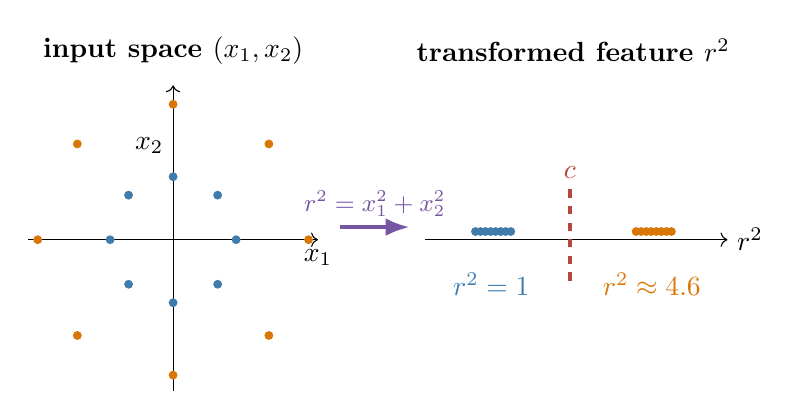
\begin{tikzpicture}[scale=0.8]
    \node[font=\bfseries] at (-3.1,3.0) {input space $(x_1,x_2)$};
    \draw[->] (-5.4,0)--(-0.8,0);
    \node[below] at (-0.8,0) {$x_1$};
    \draw[->] (-3.1,-2.4)--(-3.1,2.45);
    \node[left] at (-3.1,1.5) {$x_2$};
    \foreach \a in {0,45,...,315}{
      \fill[courseblue] ({-3.1+1.0*cos(\a)},{1.0*sin(\a)}) circle (2pt);
      \fill[courseorange] ({-3.1+2.15*cos(\a)},{2.15*sin(\a)}) circle (2pt);
    }
    \draw[-{Latex[length=3mm]},coursepurple,very thick] (-0.45,0.2)--(0.65,0.2)
      node[midway,above,font=\small] {$r^2=x_1^2+x_2^2$};
    \node[font=\bfseries] at (3.25,3.0) {transformed feature $r^2$};
    \draw[->] (0.9,0)--(5.7,0) node[right] {$r^2$};
    \foreach \x in {1.7,1.78,1.86,1.94,2.02,2.10,2.18,2.26}{\fill[courseblue] (\x,0.13) circle (2pt);}
    \foreach \x in {4.25,4.33,4.41,4.49,4.57,4.65,4.73,4.81}{\fill[courseorange] (\x,0.13) circle (2pt);}
    \draw[coursered,very thick,dashed] (3.2,-0.65)--(3.2,0.8) node[above] {$c$};
    \node[courseblue] at (1.95,-0.7) {$r^2=1$};
    \node[courseorange] at (4.5,-0.7) {$r^2\approx4.6$};
  \end{tikzpicture}

  \vspace{0.2cm}
  Now $y=0$ for $r^2<c$ and $y=1$ for $r^2>c$. A neural network learns useful feature transforms instead of requiring us to specify $r^2$ by hand.
\end{frame}

% ---------------------------------------------------------------- neuron

\begin{frame}{A Neuron: Weighted Sum, Then a Bend}
  \centering
  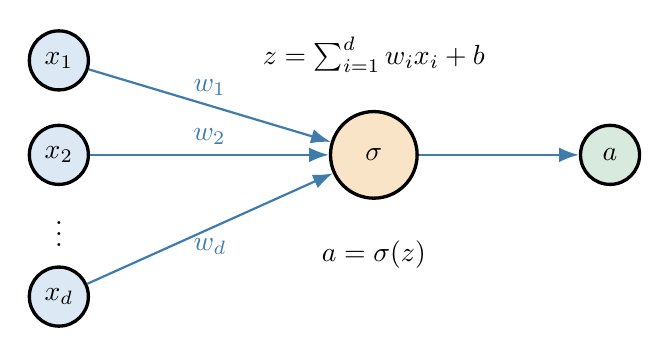
\begin{tikzpicture}[unit/.style={circle,draw,very thick,minimum size=0.75cm},
    flow/.style={-{Latex[length=2.5mm]},thick,courseblue}]
    \node[unit,fill=courselightblue] (x1) at (0,1.2) {$x_1$};
    \node[unit,fill=courselightblue] (x2) at (0,0) {$x_2$};
    \node at (0,-0.9) {$\vdots$};
    \node[unit,fill=courselightblue] (xd) at (0,-1.8) {$x_d$};
    \node[unit,fill=courselightorange,minimum size=1.1cm] (n) at (4,0) {$\sigma$};
    \node[unit,fill=coursegreen!18] (a) at (7,0) {$a$};
    \draw[flow] (x1)--(n) node[midway,above] {$w_1$};
    \draw[flow] (x2)--(n) node[midway,above] {$w_2$};
    \draw[flow] (xd)--(n) node[midway,below] {$w_d$};
    \draw[flow] (n)--(a);
    \node[above=0.35cm of n] {$z=\sum_{i=1}^{d}w_ix_i+b$};
    \node[below=0.4cm of n] {$a=\sigma(z)$};
  \end{tikzpicture}

  The circle is one neuron; incoming edges carry learned weights. The learned bias $b$ shifts its score, and the chosen nonlinear activation $\sigma$ gives its output.
\end{frame}

\begin{frame}{A Dense Layer Is Many Neurons Side by Side}
  \centering
  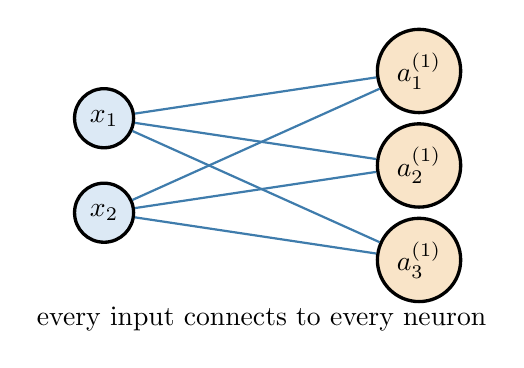
\begin{tikzpicture}[unit/.style={circle,draw,very thick,minimum size=0.75cm},edge/.style={courseblue,thick}]
    \foreach \i in {1,2}{\node[unit,fill=courselightblue] (x\i) at (0,{1.5-1.2*\i}) {$x_\i$};}
    \foreach \j in {1,2,3}{\node[unit,fill=courselightorange] (h\j) at (4,{2.1-1.2*\j}) {$a_{\j}^{(1)}$};}
    \foreach \i in {1,2}{\foreach \j in {1,2,3}{\draw[edge] (x\i)--(h\j);}}
    \node at (2,-2.25) {every input connects to every neuron};
  \end{tikzpicture}
  \[
    \mathbf z^{(1)}=\mathbf W^{(1)}\mathbf x+\mathbf b^{(1)},
    \quad\mathbf a^{(1)}=\sigma(\mathbf z^{(1)}),
    \quad\mathbf W^{(1)}\in\mathbb R^{3\times2}.
  \]
  Three neurons have three distinct weight rows and biases: $2\cdot3+3=9$ learned parameters.
\end{frame}

\begin{frame}{Layers Stack: Each One Re-describes the Data}
  \centering
  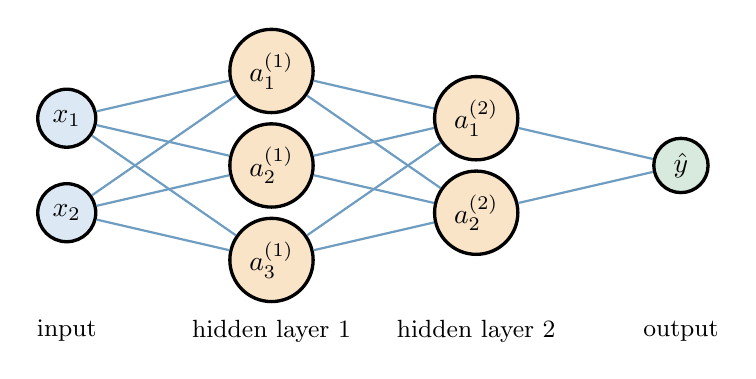
\begin{tikzpicture}[unit/.style={circle,draw,very thick,minimum size=0.65cm},edge/.style={courseblue!75,thick}]
    \foreach \i in {1,2}{\node[unit,fill=courselightblue] (x\i) at (0,{1.1-1.2*\i}) {$x_\i$};}
    \foreach \j in {1,2,3}{\node[unit,fill=courselightorange] (h\j) at (2.6,{1.7-1.2*\j}) {$a_{\j}^{(1)}$};}
    \foreach \j in {1,2}{\node[unit,fill=courselightorange] (g\j) at (5.2,{1.1-1.2*\j}) {$a_{\j}^{(2)}$};}
    \node[unit,fill=coursegreen!18] (y) at (7.8,-0.7) {$\hat y$};
    \foreach \i in {1,2}{\foreach \j in {1,2,3}{\draw[edge] (x\i)--(h\j);}}
    \foreach \i in {1,2,3}{\foreach \j in {1,2}{\draw[edge] (h\i)--(g\j);}}
    \foreach \j in {1,2}{\draw[edge] (g\j)--(y);}
    \node[font=\small] at (0,-2.8) {input}; \node[font=\small] at (2.6,-2.8) {hidden layer 1};
    \node[font=\small] at (5.2,-2.8) {hidden layer 2}; \node[font=\small] at (7.8,-2.8) {output};
  \end{tikzpicture}

  \[
    \mathbf a^{(0)}=\mathbf x,\quad
    \mathbf a^{(\ell)}=\sigma(\mathbf W^{(\ell)}\mathbf a^{(\ell-1)}+\mathbf b^{(\ell)}),\quad
    \hat y=f_{\boldsymbol\theta}(\mathbf x).
  \]
  Each circle computes one activation; later layers combine the features learned earlier.
\end{frame}

% ---------------------------------------------------------------- activations

\section{Activation Functions}
\sectiondivider{Activation Functions}

\begin{frame}{Why Layers Need a Nonlinear Activation}
  Suppose each layer is only a weighted sum, with no activation. A tiny example with one number:
  multiplying by $2$ and then by $3$ is the same as multiplying by $6$ once.

  In general two weighted-sum layers combine into one:
  \[
    \mathbf W^{(2)}\bigl(\mathbf W^{(1)}\mathbf x+\mathbf b^{(1)}\bigr)+\mathbf b^{(2)}
    =\widetilde{\mathbf W}\mathbf x+\widetilde{\mathbf b}.
  \]
  The same holds for any number of layers.

  Without an activation, a deep network is just a linear model; the activation is what makes depth useful.
\end{frame}

\begin{frame}{Sigmoid and Tanh: Smooth Squeezing Functions}
  \centering
  \begin{tikzpicture}
    \begin{axis}[width=0.9\linewidth,height=0.58\textheight,axis lines=middle,
      xmin=-5,xmax=5,ymin=-1.3,ymax=1.3,grid=both,legend style={draw=none,at={(0.02,0.98)},anchor=north west}]
      \addplot[courseorange,very thick,domain=-5:5,samples=150] {1/(1+exp(-x))};
      \addlegendentry{sigmoid}
      \addplot[coursepurple,very thick,domain=-5:5,samples=150] {tanh(x)};
      \addlegendentry{$\tanh$}
    \end{axis}
  \end{tikzpicture}
  \par\vspace{0.1cm}
  Sigmoid maps scores to $(0,1)$ (a probability-like value); $\tanh$ maps to $(-1,1)$ and is centered at 0.
  Both are flat for large $|z|$: they saturate.
\end{frame}

\begin{frame}{ReLU: Zero Below, Identity Above}
  \centering
  \begin{tikzpicture}
    \begin{axis}[width=0.9\linewidth,height=0.58\textheight,axis lines=middle,
      xmin=-5,xmax=5,ymin=-0.6,ymax=5.2,grid=both]
      \addplot[coursegreen,very thick,domain=-5:5,samples=3] {max(0,x)};
      \node[coursegreen,font=\bfseries] at (axis cs:-2.6,3.2) {$\max(0,z)$};
    \end{axis}
  \end{tikzpicture}
  \par\vspace{0.1cm}
  ReLU (rectified linear unit) outputs $0$ for negative scores and the score itself for positive ones.
  It is cheap, does not saturate for $z>0$, and is the usual choice for hidden layers.
\end{frame}

\begin{frame}{Why Saturation Hurts Learning}
  Training needs the slope of each activation: it tells how much a change in the score changes the output.
  \begin{center}
    \begin{tabular}{lcc}
      \toprule
      & steepest slope (at $z=0$) & slope for large $|z|$\\
      \midrule
      sigmoid & $0.25$ & $\approx 0.007$ at $z=5$\\
      $\tanh$ & $1$ & $\approx 0.01$ at $z=3$\\
      ReLU & $1$ & $1$ if $z>0$, $0$ if $z<0$\\
      \bottomrule
    \end{tabular}
  \end{center}
  \begin{itemize}
    \item Where the slope is almost zero, almost no learning signal flows back through the unit.
    \item ReLU has slope $1$ for positive scores, but a unit whose score stays negative has slope $0$ and learns nothing.
  \end{itemize}
  Prefer ReLU in hidden layers; keep sigmoid for outputs that must be probabilities.
\end{frame}

% ---------------------------------------------------------------- forward pass

\section{The Forward Pass}
\sectiondivider{The Forward Pass}

\begin{frame}{The Forward Pass: Compute Layer by Layer}
  \[
    \mathbf x
    \xrightarrow{\ \text{layer 1}\ }
    \mathbf a^{(1)}
    \xrightarrow{\ \text{layer 2}\ }
    \hat y
    \xrightarrow{\ \text{compare with }y\ }
    L .
  \]
  \begin{itemize}
    \item The prediction $\hat y$ comes from applying the same layer rule again and again.
    \item The target $y$ is the correct answer; the loss $L$ measures the mismatch on one example (for a whole dataset, average it).
    \item Every intermediate value is stored, because the backward pass will reuse it.
  \end{itemize}
  The forward pass turns an input into a prediction and a single loss number.
\end{frame}

\begin{frame}{Worked Forward Pass: The Numbers on the Network}
  \centering
  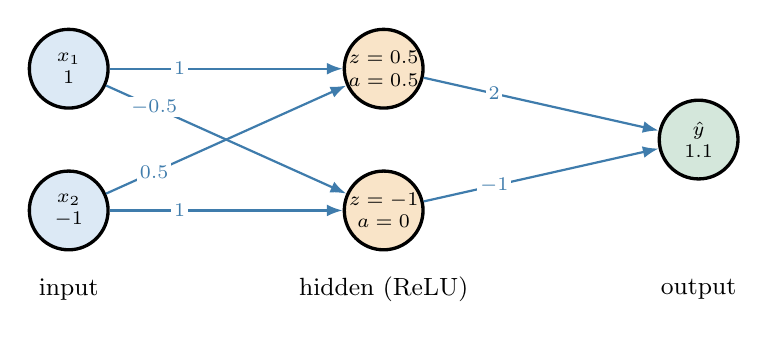
\begin{tikzpicture}[scale=1.0,
    n/.style={circle,draw,very thick,minimum size=1.0cm,inner sep=0pt,font=\scriptsize,align=center},
    w/.style={font=\scriptsize,fill=white,inner sep=1pt,pos=0.3},
    flow/.style={-{Latex[length=2mm]},thick,courseblue}]
    \node[n,fill=courselightblue] (x1) at (0,0.9) {$x_1$\\$1$};
    \node[n,fill=courselightblue] (x2) at (0,-0.9) {$x_2$\\$-1$};
    \node[n,fill=courselightorange] (h1) at (4,0.9) {$z=0.5$\\$a=0.5$};
    \node[n,fill=courselightorange] (h2) at (4,-0.9) {$z=-1$\\$a=0$};
    \node[n,fill=coursegreen!20] (y) at (8,0) {$\hat y$\\$1.1$};
    \draw[flow] (x1)--(h1) node[w]{$1$};
    \draw[flow] (x2)--(h1) node[w,pos=0.2]{$0.5$};
    \draw[flow] (x1)--(h2) node[w,pos=0.2]{$-0.5$};
    \draw[flow] (x2)--(h2) node[w]{$1$};
    \draw[flow] (h1)--(y) node[w]{$2$};
    \draw[flow] (h2)--(y) node[w]{$-1$};
    \node[font=\small] at (0,-1.9) {input};
    \node[font=\small] at (4,-1.9) {hidden (ReLU)};
    \node[font=\small] at (8,-1.9) {output};
  \end{tikzpicture}

  \vspace{0.1cm}
  Biases: $\mathbf b^{(1)}=(0,\,0.5)$ and $b^{(2)}=0.1$. Target $y=1$.
  The second hidden neuron has a negative score, so ReLU switches it off.
\end{frame}

\begin{frame}{Worked Forward Pass: The Arithmetic}
  Hidden layer ($\mathbf W^{(1)}$ has rows $(1,0.5)$ and $(-0.5,1)$):
  \[
    \mathbf z^{(1)}=\begin{bmatrix}1&0.5\\-0.5&1\end{bmatrix}
      \begin{bmatrix}1\\-1\end{bmatrix}
      +\begin{bmatrix}0\\0.5\end{bmatrix}
      =\begin{bmatrix}0.5\\-1\end{bmatrix}
  \]
  \[
    \mathbf a^{(1)}=\operatorname{ReLU}(\mathbf z^{(1)})=\begin{bmatrix}0.5\\0\end{bmatrix}.
  \]
  Output and loss, with $\mathbf w^{(2)}=(2,-1)$:
  \[
    \hat y=2\cdot0.5+(-1)\cdot0+0.1=1.1,
    \qquad
    L=\tfrac12(\hat y-y)^2=\tfrac12(0.1)^2=0.005 .
  \]
  The prediction overshoots the target by $0.1$; backpropagation will say which weights to change to fix this.
\end{frame}

\begin{frame}{The Output Layer Must Match the Task}
  \centering
  \begin{tabular}{lll}
    \toprule
    \textbf{Task} & \textbf{Output layer} & \textbf{Typical loss}\\
    \midrule
    Regression & linear, any real number & mean squared error\\
    Two classes & sigmoid, a number in $(0,1)$ & binary cross-entropy\\
    $K$ classes & softmax, $K$ probabilities & cross-entropy\\
    \bottomrule
  \end{tabular}
  \vspace{0.3cm}

  Softmax turns scores into probabilities: $\operatorname{softmax}(\mathbf z)_k=e^{z_k}/\sum_{j}e^{z_j}$.
  For scores $(2,1,0)$: $e^2\approx7.39$, $e^1\approx2.72$ and $e^0=1$ sum to $11.11$, so the probabilities are
  $(0.67,\,0.24,\,0.09)$.

  The hidden layers can be shared across tasks; only the output layer and the loss change.
\end{frame}

% ---------------------------------------------------------------- backprop

\section{Backpropagation}
\sectiondivider{Backpropagation}

\begin{frame}{Training Needs the Gradient of the Loss}
  For $P$ learned parameters, training needs all $P$ derivatives in $\nabla_{\boldsymbol\theta}L$.
  \begin{itemize}
    \item Finite differences: perturb each parameter and evaluate the loss again, costing $O(P)$ forward passes.
    \item Backpropagation: reuse local derivatives in one reverse pass to obtain all components of the gradient.
  \end{itemize}
  This reverse-mode calculation has cost comparable to a small number of forward passes for one scalar loss.
\end{frame}

\begin{frame}{A Computation Graph Splits the Work into Steps}
  \centering
  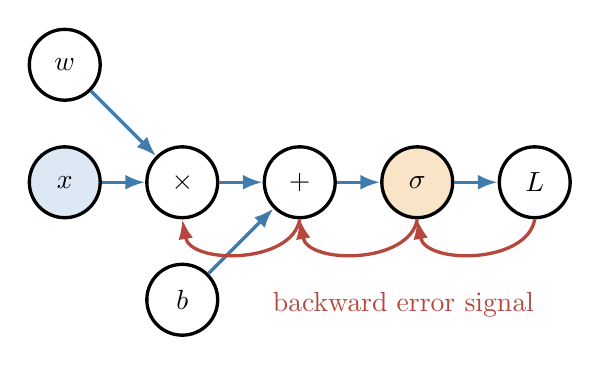
\begin{tikzpicture}[node distance=0.55cm,
    node/.style={draw,circle,minimum size=0.9cm,very thick},
    flow/.style={-{Latex[length=2.5mm]},very thick,courseblue}]
    \node[node,fill=courselightblue] (x) {$x$};
    \node[node,above=of x] (w) {$w$};
    \node[node,right=of x] (mul) {$\times$};
    \node[node,below=of mul] (b) {$b$};
    \node[node,right=of mul] (add) {$+$};
    \node[node,right=of add,fill=courselightorange] (act) {$\sigma$};
    \node[node,right=of act] (loss) {$L$};
    \draw[flow] (x)--(mul); \draw[flow] (w)--(mul); \draw[flow] (mul)--(add);
    \draw[flow] (b)--(add); \draw[flow] (add)--(act); \draw[flow] (act)--(loss);
    \draw[-{Latex[length=2.5mm]},very thick,coursered] (loss.south) to[out=-100,in=-80] (act.south);
    \draw[-{Latex[length=2.5mm]},very thick,coursered] (act.south) to[out=-100,in=-80] (add.south);
    \draw[-{Latex[length=2.5mm]},very thick,coursered] (add.south) to[out=-100,in=-80] (mul.south);
    \node[coursered] at (4.3,-1.55) {backward error signal};
  \end{tikzpicture}

  \vspace{0.2cm}
  Blue: compute values toward the loss. Red: propagate the loss derivative backward, multiplying by each operation's local derivative.
\end{frame}

\begin{frame}{The Chain Rule: Multiply the Slopes Along the Path}
  For one neuron with $z=wx+b$, $a=\sigma(z)$ and loss $L=\tfrac12(a-y)^2$, the change of $L$ with $w$ is a product of three local slopes:
  \[
    \frac{\partial L}{\partial w}
    =\underbrace{\frac{\partial L}{\partial a}}_{a-y}
     \underbrace{\frac{\partial a}{\partial z}}_{\sigma'(z)}
     \underbrace{\frac{\partial z}{\partial w}}_{x}
    =(a-y)\sigma'(z)x .
  \]
  Each factor is a slope on one edge of the computation graph. At a branch, add the derivatives contributed by all paths.
\end{frame}

\begin{frame}{Layer Error Signals Are Passed Backward}
  \centering
  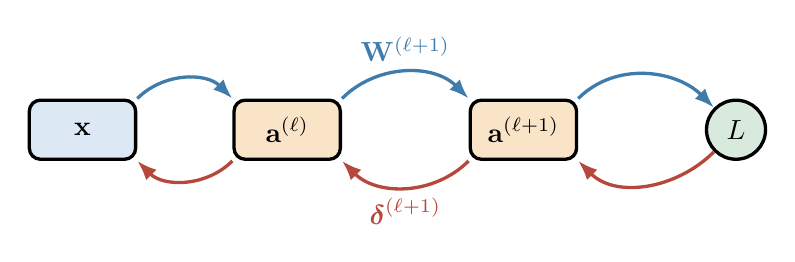
\begin{tikzpicture}[layerbox/.style={draw,rounded corners,very thick,minimum height=0.75cm,minimum width=1.35cm},
    unit/.style={circle,draw,very thick,minimum size=0.75cm},
    forward/.style={-{Latex[length=2.5mm]},courseblue,very thick},
    backward/.style={-{Latex[length=2.5mm]},coursered,very thick}]
    \node[layerbox,fill=courselightblue] (x) at (0,0) {$\mathbf x$};
    \node[layerbox,fill=courselightorange] (h) at (2.6,0) {$\mathbf a^{(\ell)}$};
    \node[layerbox,fill=courselightorange] (g) at (5.6,0) {$\mathbf a^{(\ell+1)}$};
    \node[unit,fill=coursegreen!18] (loss) at (8.3,0) {$L$};
    \draw[forward] (x.north east) to[out=45,in=135] (h.north west);
    \draw[forward] (h.north east) to[out=45,in=135] node[above] {$\mathbf W^{(\ell+1)}$} (g.north west);
    \draw[forward] (g.north east) to[out=45,in=135] (loss.north west);
    \draw[backward] (loss.south west) to[out=-135,in=-45] (g.south east);
    \draw[backward] (g.south west) to[out=-135,in=-45] node[below] {$\boldsymbol\delta^{(\ell+1)}$} (h.south east);
    \draw[backward] (h.south west) to[out=-135,in=-45] (x.south east);
  \end{tikzpicture}
  \[
    \delta_j^{(\ell)}=\frac{\partial L}{\partial z_j^{(\ell)}}
      =\sigma'(z_j^{(\ell)})
       \sum_k W_{kj}^{(\ell+1)}\delta_k^{(\ell+1)}.
  \]
  The sum collects every path from neuron $j$ to the next layer. In vector form:
  \[
    \boldsymbol\delta^{(\ell)}
    =\left(\mathbf W^{(\ell+1)}\right)^\top
      \boldsymbol\delta^{(\ell+1)}
      \odot\sigma'(\mathbf z^{(\ell)}).
  \]
  Here $\odot$ multiplies entries; for squared error and a linear output, $\delta^{(M)}=\hat y-y$.
\end{frame}

\begin{frame}{From Error Signals to Weight Gradients}
  A weight $W_{ji}^{(\ell)}$ connects activation $a_i^{(\ell-1)}$ to neuron $j$:
  \[
    \boxed{
    \frac{\partial L}{\partial\mathbf W^{(\ell)}}
      =\boldsymbol\delta^{(\ell)}\bigl(\mathbf a^{(\ell-1)}\bigr)^\top},
    \qquad
    \boxed{\frac{\partial L}{\partial\mathbf b^{(\ell)}}
      =\boldsymbol\delta^{(\ell)}} .
  \]
  \begin{itemize}
    \item Entrywise: $\partial L/\partial W_{ji}^{(\ell)}=\delta_j^{(\ell)}a_i^{(\ell-1)}$.
    \item For a mini-batch, average each example's outer-product gradient.
  \end{itemize}
  Stored forward activations and backward error signals are sufficient for this layer's gradients.
\end{frame}

\begin{frame}{Worked Backward Pass: Output Layer}
  From the forward pass, $\hat y-y=0.1$ and $\mathbf a^{(1)}=(0.5,0)$.
  \[
    \delta^{(2)}=\hat y-y=0.1,
    \quad
    \frac{\partial L}{\partial\mathbf w^{(2)}}
      =0.1\begin{bmatrix}0.5\\0\end{bmatrix}
      =\begin{bmatrix}0.05\\0\end{bmatrix},
    \quad
    \frac{\partial L}{\partial b^{(2)}}=0.1 .
  \]
  \begin{itemize}
    \item The first hidden neuron was active ($a=0.5$), so its output weight gets a gradient.
    \item The second was off ($a=0$), so its output weight gets none.
  \end{itemize}
  Positive gradients say that lowering these weights and the bias reduces the overshoot.
\end{frame}

\begin{frame}{Worked Backward Pass: Hidden Layer}
  Send $\delta^{(2)}=0.1$ back through $\mathbf w^{(2)}=(2,-1)$, then multiply by the ReLU slopes $(1,0)$
  (slope $1$ where $z>0$, slope $0$ where $z<0$):
  \[
    \boldsymbol\delta^{(1)}
    =\begin{bmatrix}2\\-1\end{bmatrix}0.1\odot\begin{bmatrix}1\\0\end{bmatrix}
    =\begin{bmatrix}0.2\\-0.1\end{bmatrix}\odot\begin{bmatrix}1\\0\end{bmatrix}
    =\begin{bmatrix}0.2\\0\end{bmatrix}.
  \]
  The inactive neuron receives no error signal: ReLU blocks it.
  Its weights will therefore get no gradient on this example.
\end{frame}

\begin{frame}{Worked Backward Pass: Hidden-Layer Gradients}
  With $\boldsymbol\delta^{(1)}=(0.2,0)$ and the input $\mathbf x=(1,-1)$:
  \[
    \frac{\partial L}{\partial\mathbf W^{(1)}}
    =\boldsymbol\delta^{(1)}\mathbf x^\top
    =\begin{bmatrix}0.2\\0\end{bmatrix}
      \begin{bmatrix}1&-1\end{bmatrix}
    =\begin{bmatrix}0.2&-0.2\\0&0\end{bmatrix},
  \]
  \[
    \frac{\partial L}{\partial\mathbf b^{(1)}}
    =\begin{bmatrix}0.2\\0\end{bmatrix}.
  \]
  A positive entry means ``lower this weight'', a negative one ``raise it'': the prediction $1.1$ is too high, and these gradients push it down.
  Only the active neuron and the weights it used are blamed for the error.
\end{frame}

\begin{frame}{Training Alternates Differentiation and Optimization}
  \centering
  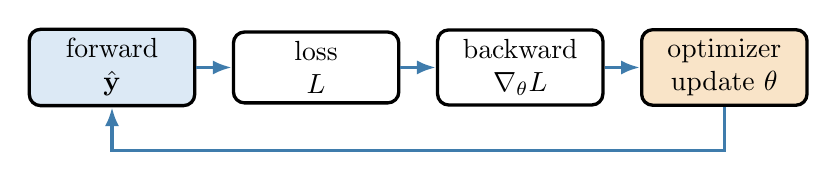
\begin{tikzpicture}[node distance=0.45cm,
    box/.style={draw,rounded corners,minimum width=2.1cm,minimum height=0.85cm,very thick,align=center},
    flow/.style={-{Latex[length=2.4mm]},very thick,courseblue}]
    \node[box,fill=courselightblue] (forward) {forward\\$\hat{\mathbf y}$};
    \node[box,right=of forward] (loss) {loss\\$L$};
    \node[box,right=of loss] (backward) {backward\\$\nabla_\theta L$};
    \node[box,fill=courselightorange,right=of backward] (update) {optimizer\\update $\theta$};
    \draw[flow] (forward)--(loss); \draw[flow] (loss)--(backward); \draw[flow] (backward)--(update);
    \draw[flow] (update.south) -- ++(0,-0.55) -| (forward.south);
  \end{tikzpicture}

  \vspace{0.2cm}
  One round: predict, measure the loss, compute all gradients, move the parameters a small step; repeat on the next mini-batch.
  The optimization lecture covers how large that step should be.

  Backpropagation only computes gradients; the optimizer decides how to use them.
\end{frame}

% ---------------------------------------------------------------- capacity

\section{What Networks Can Represent}
\sectiondivider{What Networks Can Represent}

\begin{frame}{How ReLU Units Build a Curve}
  \centering
  \begin{tikzpicture}
    \begin{axis}[width=0.92\linewidth,height=0.58\textheight,xmin=-3.2,xmax=3.2,ymin=-1.3,ymax=1.3,
      axis lines=middle,grid=both,legend style={draw=none,at={(0.03,0.97)},anchor=north west}]
      \addplot[courseblue,very thick,domain=-3.14:3.14,samples=160] {sin(deg(x))};
      \addlegendentry{$f(x)=\sin x$}
      \addplot[courseorange,very thick,mark=*] coordinates {
        (-3.14,0) (-2.36,-0.707) (-1.57,-1) (-0.79,-0.707) (0,0)
        (0.79,0.707) (1.57,1) (2.36,0.707) (3.14,0)};
      \addlegendentry{ReLU network}
    \end{axis}
  \end{tikzpicture}
  \par\vspace{0.1cm}
  Each hidden ReLU adds one bend; the output layer adds the pieces with weights.
  In one input dimension, a one-hidden-layer ReLU network can reproduce any piecewise-linear curve using about one hidden unit per bend.
  More hidden units give more bends and a closer fit to a smooth curve.
\end{frame}

\begin{frame}{Universal Approximation: Existence, Not Learning}
  For continuous $f$ on compact $K\subset\mathbb R^d$ and any $\varepsilon>0$,
  a \emph{single hidden layer} of sufficient width $N$ can satisfy
  \[
    \sup_{\mathbf x\in K}\left|f(\mathbf x)-
      \left(c+\sum_{j=1}^{N}\alpha_j
        \operatorname{ReLU}(\mathbf w_j^\top\mathbf x+b_j)\right)\right|<\varepsilon.
  \]
  This existence result does not specify:
  \begin{itemize}
    \item the required width or how to find the weights;
    \item whether training is stable or data-efficient;
    \item behavior beyond $K$ or on unseen data.
  \end{itemize}
  Approximation capacity alone does not select an architecture or establish generalization.
\end{frame}

\appendix

\sectiondivider{Appendix: optional depth}

\begin{frame}{Forward Mode Versus Reverse Mode}
  The Jacobian $J_{ij}=\partial y_i/\partial x_j$ contains all input--output derivatives.
  \[
    \underbrace{\mathbf J_f\mathbf v}_{\text{forward: one input direction}}
    \qquad\qquad
    \underbrace{\mathbf u^\top\mathbf J_f}_{\text{reverse: one output weighting}}.
  \]
  A scalar loss has one output and many parameters. Reverse mode with $\mathbf u=1$ returns $\nabla_{\boldsymbol\theta}L$ in one pass; forward mode needs one direction per parameter.
\end{frame}

\begin{frame}{Finite Differences Check a Gradient}
  For coordinate $j$ and unit vector $\mathbf e_j$,
  \[
    \frac{\partial L}{\partial\theta_j}
    \approx
    \frac{L(\boldsymbol\theta+h\mathbf e_j)-L(\boldsymbol\theta-h\mathbf e_j)}{2h}
    \qquad\text{with error }O(h^2).
  \]
  \begin{itemize}
    \item Large $h$: truncation error hides local behavior.
    \item Tiny $h$: floating-point cancellation dominates.
    \item Nondifferentiable activation points require care.
  \end{itemize}
  This is a debugging check on a few coordinates, not a way to train: it costs two forward passes per parameter.
\end{frame}

\begin{frame}{Initialization Tries to Preserve Signal Scale}
  Suppose inputs and centered weights are independent. For fan-in $d_{\ell-1}$ (the number of inputs of a neuron),
  \[
    \operatorname{Var}(z_i^{(\ell)})
    \approx d_{\ell-1}\operatorname{Var}(W_{ij}^{(\ell)})
      \operatorname{Var}(a_j^{(\ell-1)}).
  \]
  \begin{itemize}
    \item Xavier: $\operatorname{Var}(W_{ij})\approx 1/d_{\ell-1}$ for roughly symmetric activations.
    \item He: $\operatorname{Var}(W_{ij})\approx 2/d_{\ell-1}$ compensates for inactive ReLU units.
  \end{itemize}
  These are variance heuristics, not guarantees: they keep activations from shrinking or blowing up at the start of training.
\end{frame}

\begin{frame}{Derivative Information Can Constrain the Learned Function}
  If derivative targets $\mathbf g_i\approx\nabla f(\mathbf x_i)$ are available, use
  \[
    L(\boldsymbol\theta)
    =\frac1n\sum_{i=1}^n|f_{\boldsymbol\theta}(\mathbf x_i)-y_i|^2
    +\lambda\frac1n\sum_{i=1}^n
      \|\nabla_{\mathbf x}f_{\boldsymbol\theta}(\mathbf x_i)-\mathbf g_i\|_2^2.
  \]
  Function values anchor height; derivatives constrain local shape. The weight $\lambda$ balances the two terms.
  This Sobolev-style objective helps only when derivative information is reliable and consistently scaled.
\end{frame}

\end{document}
